% **************************************************
% Document Class Definition
% **************************************************
\documentclass[%
	paper=A4,					% paper size --> A4 is default in Germany
	twoside=true,				% onesite or twoside printing
	openright,					% doublepage cleaning ends up right side
	parskip=full,				% spacing value / method for paragraphs
	chapterprefix=true,			% prefix for chapter marks
	11pt,						% font size
	headings=normal,			% size of headings
	bibliography=totoc,			% include bib in toc
	listof=totoc,				% include listof entries in toc
	titlepage=on,				% own page for each title page
	captions=tableabove,		% display table captions above the float env
	draft=false,				% value for draft version
]{scrreprt}%

% **************************************************
% Debug LaTeX Information
% **************************************************
%\listfiles

% **************************************************
% Information and Commands for Reuse
% **************************************************
\newcommand{\reqTitle}{Collectd Requirements Specification}
\newcommand{\reqName}{\Large{Jonathan Reyna} \\
	\small{Resident Consultant}\\[-1mm]
	\small{Juniper Networks, Inc.}\\
	\Large{Shane Coury} \\
	\small{Network Engineering Operations Manager} \\[-1mm]
	\small{Wide Open West, Inc.}
}

\newcommand{\reqSubject}{Application Development}
\newcommand{\reqDate}{\today}
\newcommand{\reqSpecVersion}{0.1}

\newcommand{\firstReviewer}{Brian Nabors II}
\newcommand{\firstReviewerTitle}{Network Engineer}
\newcommand{\firstReviewerDepartment}{Operations}
\newcommand{\firstReviewerCompany}{\protect{Wide Open West, Inc.}}

\newcommand{\secondReviewer}{Lamoni Finlayson}
\newcommand{\secondReviewerTitle}{\protect{Resident Engineer}}
\newcommand{\secondReviewerDepartment}{Advanced Services}
\newcommand{\secondReviewerCompany}{\protect{Juniper Networks, Inc.}}

\newcommand{\thesisFirstSupervisor}{Shane Coury}
\newcommand{\thesisSecondSupervisor}{Paul Dietl}

\newcommand{\thesisUniversity}{\protect{Wide Open West, Inc.}}
\newcommand{\thesisUniversityDepartment}{Operations}
\newcommand{\thesisUniversityInstitute}{Institut for Clean Thesis Dev}
\newcommand{\thesisUniversityGroup}{Network Engineering}
\newcommand{\thesisUniversityCity}{Alpharetta}
\newcommand{\thesisUniversityStreetAddress}{11675 Rainwater Drive}
\newcommand{\thesisUniversityPostalCode}{30009}

% **************************************************
% Load and Configure Packages
% **************************************************
\usepackage[utf8]{inputenc}		% defines file's character encoding
\usepackage[english]{babel} % babel system, adjust the language of the content
\usepackage[					% clean thesis style
	figuresep=colon,%
	sansserif=false,%
	hangfigurecaption=false,%
	hangsection=true,%
	hangsubsection=true,%
	colorize=full,%
	colortheme=bluemagenta,%
	bibsys=bibtex,%
	bibfile=bib-refs,%
	bibstyle=alphabetic,%
]{cleanthesis}
\usepackage{enumerate}
					% setup the hyperref-package options
\hypersetup{pdftitle={\reqTitle},	% 	- title (PDF meta)
	pdfsubject={\reqSubject},% 	- subject (PDF meta)
	pdfauthor={\reqName},	% 	- author (PDF meta)
	plainpages=false,			% 	-
	colorlinks=false,			% 	- colorize links?
	pdfborder={0 0 0},			% 	-
	breaklinks=true,			% 	- allow line break inside links
	bookmarksnumbered=true,		%
	bookmarksopen=true			%
}

% **************************************************
% Document CONTENT
% **************************************************
\begin{document}

% --------------------------
% rename document parts
% --------------------------
%\renewcaptionname{ngerman}{\figurename}{Abb.}
%\renewcaptionname{ngerman}{\tablename}{Tab.}
\renewcaptionname{english}{\figurename}{Fig.}
\renewcaptionname{english}{\tablename}{Tab.}

% --------------------------
% Front matter
% --------------------------
\pagenumbering{roman}			% roman page numbing (invisible for empty page style)
\pagestyle{empty}				% no header or footers
% !TEX root = ../thesis-example.tex
%
% ------------------------------------  --> cover title page
\begin{titlepage}
	\pdfbookmark[0]{Cover}{Cover}
	\centering
	\hfill
	\vfill
	{\LARGE\thesisTitle\par}
	\rule[5pt]{\textwidth}{.4pt} \par
	{\thesisName}
	\vfill
	\large\thesisDate\\
	Version: \reqSpecVersion{}
\end{titlepage}


% ------------------------------------  --> main title page
\begin{titlepage}
	\pdfbookmark[0]{Titlepage}{Titlepage}
	\tgherosfont{}
	\centering

	{\Large \thesisUniversity} \\[4mm]
	
\includegraphics[width=4cm]{gfx/wide_open_west_logo_white_bg} \\[2mm]
	\textsf{\thesisUniversityGroup} \\
	\textsf{\thesisUniversityDepartment} \\
	%	\textsf{\thesisUniversityInstitute} \\


	\vfill
	{\large \thesisSubject} \\[5mm]
	{\LARGE \color{ctcolortitle}\textbf{\thesisTitle} \\[10mm]}
	{\Large \thesisName} \\

	\vfill
	\begin{minipage}[t]{.27\textwidth}
		\raggedleft{}
		\textit{1. Reviewer}
	\end{minipage}
	\hspace*{15pt}
	\begin{minipage}[t]{.65\textwidth}
		{\Large \thesisFirstReviewer} \\
		{\small \thesisFirstReviewerTitle} \\[-1mm]
		{\small \thesisFirstReviewerDepartment} \\[-1mm]
		{\small \thesisFirstReviewerUniversity}
	\end{minipage} \\[5mm]
	\begin{minipage}[t]{.27\textwidth}
		\raggedleft{}
		\textit{2. Reviewer}
	\end{minipage}
	\hspace*{15pt}
	\begin{minipage}[t]{.65\textwidth}
		{\Large \thesisSecondReviewer} \\
		{\small \thesisSecondReviewerTitle} \\[-1mm]
		{\small \thesisSecondReviewerDepartment} \\[-1mm]
		{\small \thesisSecondReviewerUniversity}
	\end{minipage} \\[10mm]
	\begin{minipage}[t]{.27\textwidth}
		\raggedleft{}
		\textit{Supervisors}
	\end{minipage}
	\hspace*{15pt}
	\begin{minipage}[t]{.65\textwidth}
		\thesisFirstSupervisor\ and \thesisSecondSupervisor{}
	\end{minipage} \\[10mm]

	\thesisDate\\

\end{titlepage}


% ------------------------------------  --> lower title back for single page layout
\hfill
\vfill
{\small
	\textbf{\thesisName} \\
	\textit{\thesisTitle} \\
	\thesisSubject, \thesisDate\\
	Reviewers: \thesisFirstReviewer\ and \thesisSecondReviewer\\
	Supervisors: \thesisFirstSupervisor\ and \thesisSecondSupervisor\\[1.5em]
	\textbf{\thesisUniversity} \\
	\textit{\thesisUniversityGroup} \\
	\thesisUniversityInstitute\\
	\thesisUniversityDepartment\\
	\thesisUniversityStreetAddress\\
	\thesisUniversityPostalCode\ and \thesisUniversityCity{}
}
		% INCLUDE: all titlepages
\cleardoublepage{}

\pagestyle{plain}				% display just page numbers
% !TEX root = ../main.tex
%
\pdfbookmark[0]{Abstract}{Abstract}
\chapter*{Abstract}
\label{sec:abstract}
\vspace*{-10mm}

\blindtext{}

\vspace*{20mm}

{\usekomafont{chapter}Abstract (different language)}\label{sec:abstract-diff} \\

\blindtext{}
		% INCLUDE: the abstracts (english and german)
\cleardoublepage{}
%
% !TEX root = ../thesis-example.tex
%
\pdfbookmark[0]{Acknowledgement}{Acknowledgement}
\chapter*{Acknowledgement}
\label{sec:acknowledgement}
\vspace*{-10mm}

\Blindtext[2][2]
 % INCLUDE: acknowledgement
\cleardoublepage{}
%
\setcounter{tocdepth}{2}		% define depth of toc
\tableofcontents				% display table of contents
\cleardoublepage{}

% --------------------------
% Body matter
% --------------------------
\pagenumbering{arabic}			% arabic page numbering
\setcounter{page}{1}			% set page counter
\pagestyle{maincontentstyle} 	% fancy header and footer

% !TEX root = ../main.tex
%
\chapter{Introduction}\label{sec:intro}

\cleanchapterquote{The art of programming is the art of organizing complexity,
of mastering multitude and avoiding its bastard chaos as effectively as 
possible}{E. W. Dijkstra}{(Computer Science Pioneer)}

Modern network automation is generally achieved using a group of small to medium
sized software programs developed in isolation of each other. Dispite their isolation,
most programs have the same general flow of logic. Almost every network automation
tool can be described on a high level with these simple steps.
\begin{figure}[h]
\begin{minipage}{.5\textwidth}
	\begin{enumerate}
		\item Get the data from devices that contains the answer to a 
			question of interest. The answer, at least in part, 
			satisfies a business requirement.
		\item Take steps to convert the raw data into information. 
			Common steps used to convert the data include the 
			following:
			\begin{itemize}[noitemsep]
				\item Isolate specific data points of interest.
				\item Convert data points to strong types for 
					safe comparison operations.
				\item Compare parsed data with other gathered 
					data or constant values to answer a 
					question of interest.
			\end{itemize}
		\item Perform some action based on the answer to the question 
			of interest. Common actions include the following:
			\begin{itemize}[noitemsep]
				\item Update a webpage.
				\item Send an email.
				\item Configure a device.
			\end{itemize}
	\end{enumerate}
\end{minipage}
\begin{minipage}{0.5\textwidth}
	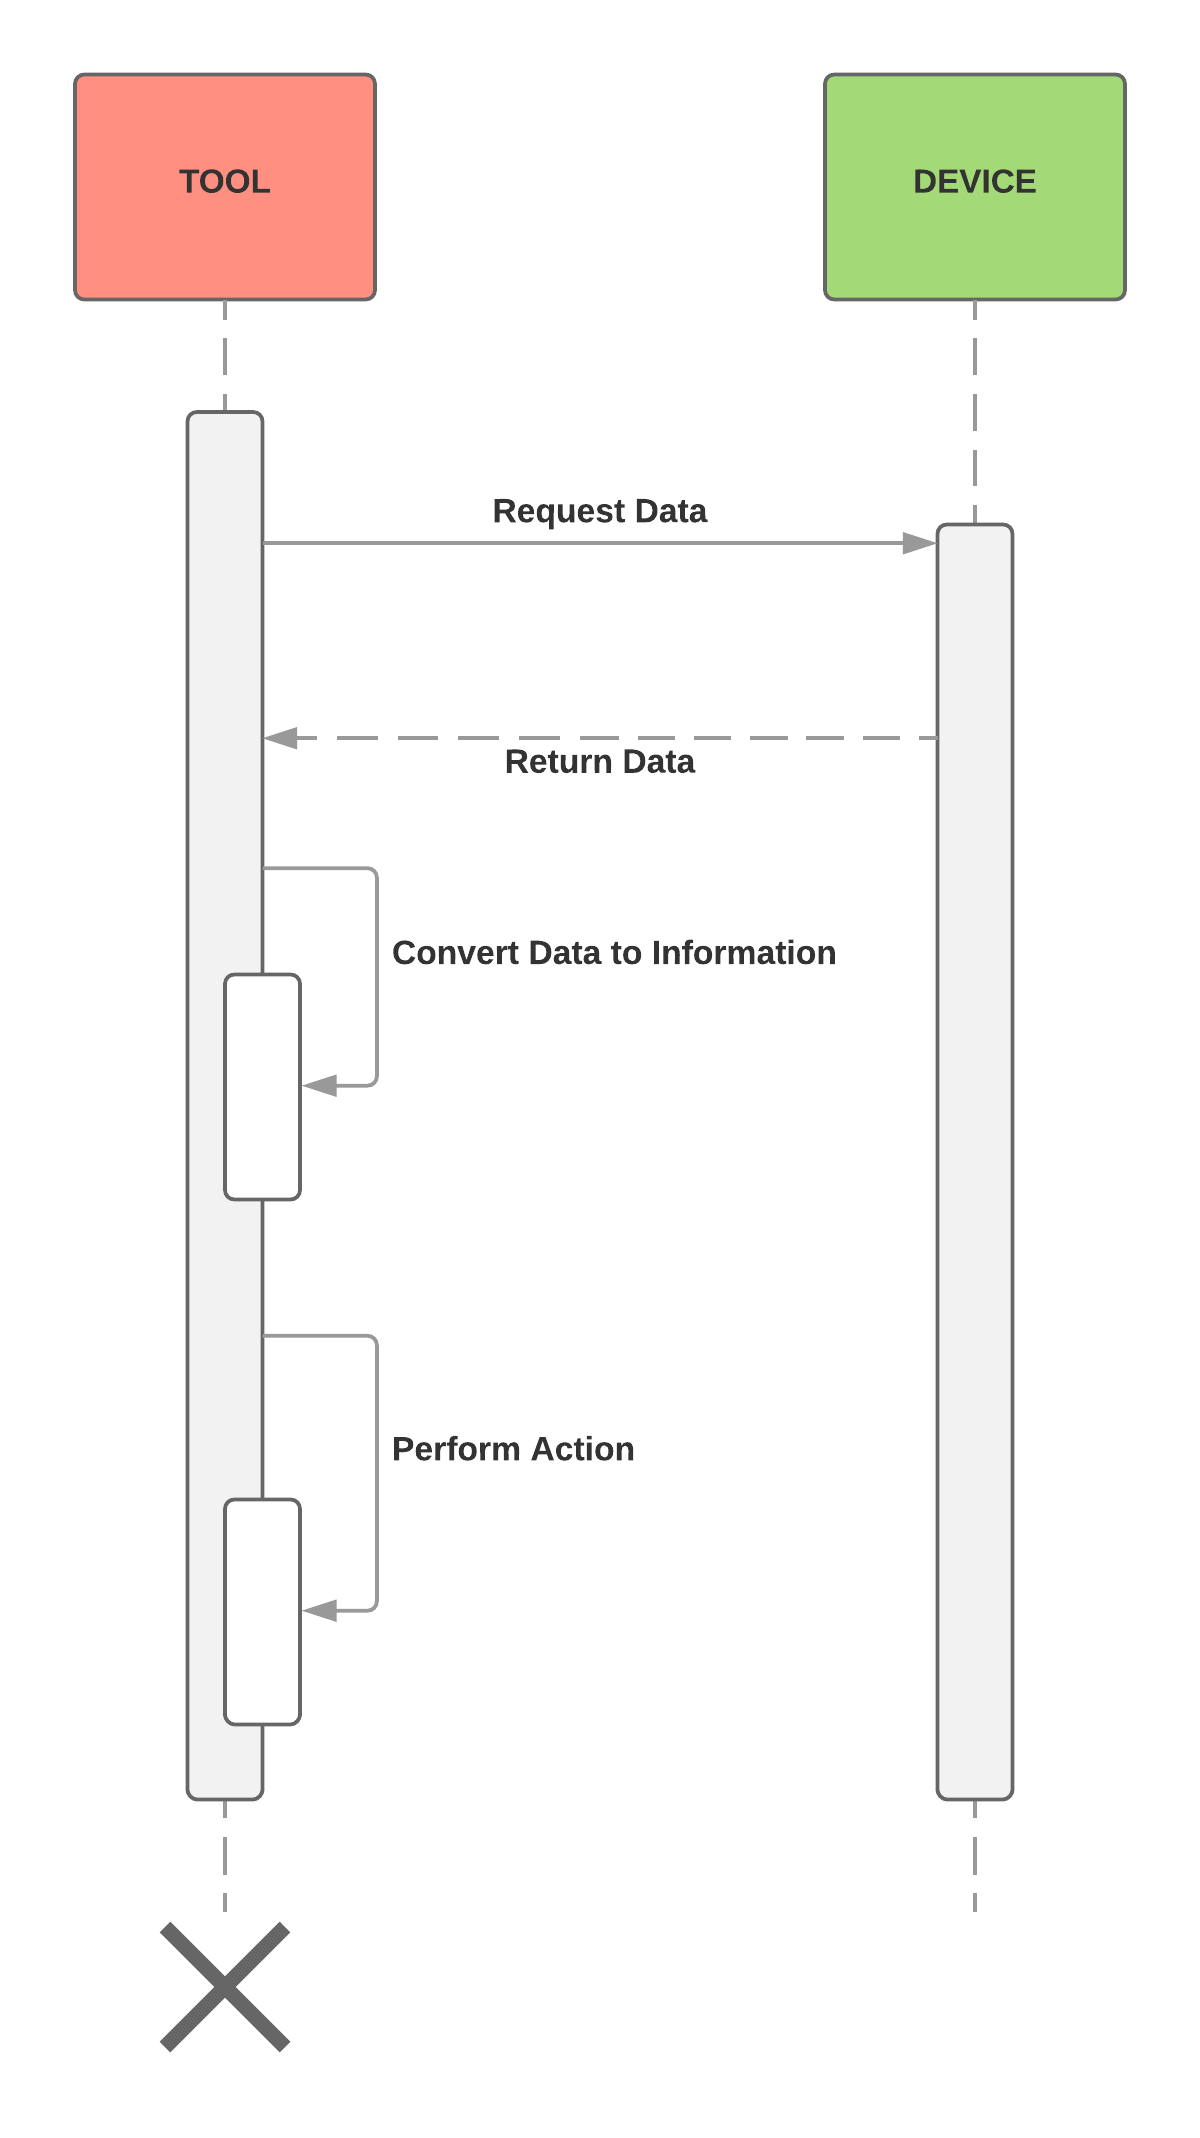
\includegraphics[width=\textwidth]{gfx/general_tool_logic_flow}
\end{minipage}
\end{figure}

The inventory tool has logic that is easy to understand, and can serve as a 
concrete example of the logic flow above. During step 1, the inventory tool
uses NETCONF over SSH to run the show chassis hardware detail command, which
provides the inventory data required. Step 2 is achieved by storing the inventory
data in a relational database. Finally, in step 3, the tool answers user queries 
A quick analysis of the inventory tool can 
A concrete example can serve to illustrate the above logic flow.
\section{Postcards: My Address}
\label{sec:intro:address}

\textbf{Ricardo Langner} \\
Alfred-Schrapel-Str. 7 \\
01307 Dresden \\
Germany


\section{Motivation and Problem Statement}
\label{sec:intro:motivation}

blah blah blah
In light of the first two steps in the general flow of logic, one only needs a
trivial example to show how this and that each 
project is developed in isolation, it's easy to see how 
In 
There are at least two approaches to remedy these inefficiencies. 

Modern network automation is typically implemented as a small or medium sized
software program that answers questions about, or changes the state of, a 
network. Conventional projects 
A network automation project, loosely defined, is a small to medium sized 
software program that answers questions about, or change the state of, 
a network. Conventional practices isolate their development lifecycle
from other projects. In part, the isolation is desireable for maximum flexibility in the 
implementation. Developers aren't constrained by design limitations of previous
projects, and can make the best descisions for the project at hand. That 
flexibility, however, comes at a cost: effort duplication. 

Effort duplication is most noticible in the data collection code required 
by most network automation tools. Since projects are deveoped in isolation, 
sharing data with other applications is an afterthought. Code, data,
compute, maintenance, and programming effort is often duplicated. There are at least
two approaches to remedy these inefficiencies. 

The first enforces strict rules on the development lifecycle. New rules
would require every project to consider every other project in its design phase. 
The flexibility of an isolated project is sacrified for global design consistency.
At best, project design complexity would increase on a linear scale, and 
exponentially in the worst case.

A more practical approach would adapt an architectural pattern to the to the 
existing development lifecycle. The pattern would eliminate duplication
efforts by consolidating homogenous logic to make the results available to
client applications. Collectd is an instance of this pattern. 

Collectd is responsible for collecting, storing, relating, and providing data retrieved 
from network devices to client applications. It consolidates all data 
collection logic, alleviating client applications of that responsibility.
When a tool needs data, it simply requests it from collectd. 

Collectd has numerous advantages over an isolated project's data collection approach. 
Client applications no longer need collection code, making them easier to reason
about, and faster to enhance, maintain, test, and document. Collection code will
be more stable and robust, because writing collection code will be concentrated,
instead of duplicated. Without the inefficiencies of a strict lifecycle approach, 
applications will maintain maximum flexibility to satisfy business requirements.
There will be fine grained control over SSH sessions to devices. Collectd will
have a global perspective of collected data from all applications, and the 
relationships between that data, which offers unique potential to answer 
questions that have not yet been considered, or were thought impractical to 
answer.
\Blindtext[3][1]~\cite{Jurgens:2000,Jurgens:1995,Miede:2011,Kohm:2011,Apple:keynote:2010,Apple:numbers:2010,Apple:pages:2010}

\section{Results}
\label{sec:intro:results}

\Blindtext[1][2]

\subsection{Some References}
\label{sec:intro:results:refs}
\cite{WEB:GNU:GPL:2010,WEB:Miede:2011}

\section{Thesis Structure}
\label{sec:intro:structure}

\textbf{Chapter~\ref{sec:related}} \\[0.2em]
\blindtext{}

\textbf{Chapter~\ref{sec:system}} \\[0.2em]
\blindtext{}

\textbf{Chapter~\ref{sec:concepts}} \\[0.2em]
\blindtext{}

\textbf{Chapter~\ref{sec:concepts}} \\[0.2em]
\blindtext{}

\textbf{Chapter~\ref{sec:conclusion}} \\[0.2em]
\blindtext{}
 % INCLUDE: introduction
% !TEX root = ../main.tex
%
\chapter{Related Work}
\label{sec:related}

\cleanchapterquote{A picture is worth a thousand words. An interface is worth a thousand pictures.}{Ben Shneiderman}{(Professor for Computer Science)}

\Blindtext[2][1]

\section{Related Work Section 1}
\label{sec:related:sec1}

\Blindtext[2][2]

\section{Related Work Section 2}
\label{sec:related:sec2}

\Blindtext[3][2]

\section{Related Work Section 3}
\label{sec:related:sec3}

\Blindtext[4][2]

\section{Conclusion}
\label{sec:related:conclusion}

\Blindtext[2][1]
 % INCLUDE: related work
% !TEX root = ../thesis-example.tex
%
\chapter{System}
\label{sec:system}

\cleanchapterquote{Innovation distinguishes between a leader and a follower.}{Steve Jobs}{(CEO Apple Inc.)}

\Blindtext[2][1]

\section{System Section 1}
\label{sec:system:sec1}

\Blindtext[1][2]

\begin{figure}[htb]
	
\includegraphics[width=\textwidth]{gfx/Clean-Thesis-Figure}
	\caption{Figure example: \textit{(a)} example part one, \textit{(c)} example part two; \textit{(c)} example part three\label{fig:system:example1}}
\end{figure}

\Blindtext[1][2]

\section{System Section 2}
\label{sec:system:sec2}

\Blindtext[1][2]

\begin{figure}[htb]
	
\includegraphics[width=\textwidth]{gfx/Clean-Thesis-Figure}
	\caption{Another Figure example: \textit{(a)} example part one, \textit{(c)} example part two; \textit{(c)} example part three\label{fig:system:example2}}
\end{figure}

\Blindtext[2][2]

\section{System Section 3}
\label{sec:system:sec3}

\Blindtext[4][2]

\section{Conclusion}
\label{sec:system:conclusion}

\Blindtext[2][1]
	% INCLUDE: system
% !TEX root = ../main.tex
%
\chapter{Concepts: This text is here to test a very long title, to simulate the line break behavior, to show that an extremely long tilte also works}
\label{sec:concepts}

\cleanchapterquote{Users do not care about what is inside the box, as long as the box does what they need done.}{Jef Raskin}{about Human Computer Interfaces}

\Blindtext[2][1]

\section{Concepts Section 1}
\label{sec:concepts:sec1}

\Blindtext[2][2]

\section{Concepts Section 2}
\label{sec:concepts:sec2}

\Blindtext[3][2]

\section{Concepts Section 3}
\label{sec:concepts:sec3}

\Blindtext[4][2]

\section{Conclusion}
\label{sec:concepts:conclusion}

\Blindtext[2][1]
 % INCLUDE: concepts
% !TEX root = ../main.tex
%
\chapter{Conclusion}
\label{sec:conclusion}

\Blindtext[2][1]

\section{System Section 1}
\label{sec:conclusion:sec1}

\Blindtext[2][2]

\section{System Section 2}
\label{sec:conclusion:sec2}

\Blindtext[3][2]

\section{Future Work}
\label{sec:conclusion:future}

\Blindtext[2][2]
 % INCLUDE: conclusion
\cleardoublepage{}

% --------------------------
% Back matter
% --------------------------
{%
	\setstretch{1.1}
	\renewcommand{\bibfont}{\normalfont\small}
	\setlength{\biblabelsep}{0pt}
	\setlength{\bibitemsep}{0.5\baselineskip plus 0.5\baselineskip}
	\printbibliography[nottype=online]
	\printbibliography[heading=subbibliography,title={Webseiten},type=online,prefixnumbers={@}]
}
\cleardoublepage{}

\listoffigures
\cleardoublepage{}

\listoftables
\cleardoublepage{}

% !TEX root = ../thesis-example.tex
%
\pagestyle{empty}
\hfill
\vfill
\pdfbookmark[0]{Colophon}{Colophon}
\section*{Colophon}

This thesis was typeset with \LaTeXe.
It uses the \textit{Clean Thesis} style developed by Ricardo Langner.
The design of the \textit{Clean Thesis} style is inspired by user guide documents from Apple Inc.

Download the \textit{Clean Thesis} style at \url{http://cleanthesis.der-ric.de/}.

\cleardoublepage{}

% !TEX root = ../thesis-example.tex
%
%************************************************
% Declaration
%************************************************
\pdfbookmark[0]{Declaration}{Declaration}
\chapter*{Declaration}
\label{sec:declaration}
\thispagestyle{empty}

You can put your declaration here, to declare that you have completed your work solely and only with the help of the references you mentioned.

\bigskip

\noindent\textit{\clientCompanyCity, \reqDate}

\smallskip

\begin{flushright}
	\begin{minipage}{5cm}
		\rule{\textwidth}{1pt}
		\centering\reqName{}
	\end{minipage}
\end{flushright}

%*****************************************
%*****************************************

\clearpage
\newpage
\mbox{}

% **************************************************
% End of Document CONTENT
% **************************************************
\end{document}
